\documentclass{cmc}

\begin{document}

\pagestyle{fancy}
\lhead{\textit{\textbf{Computational Motor Control, Spring 2025} \\
    Python exercise, Lab 1, NOT GRADED}} \rhead{Student \\ Names}

\section*{Student names: \ldots (please update)}

\textit{Instructions: Update this file (or recreate a similar one, e.g.\ in
  Word) to prepare your answers to the questions. Feel free to add text,
  equations and figures as needed. Hand-written notes, e.g.\ for the development
  of equations, can also be included e.g.\ as pictures (from your cell phone or
  from a scanner).  \textbf{This lab is not graded. However, the lab exercises
    are meant as a way to familiarise with dynamical systems and to study them
    using Python to prepare you for the final project.} This file does not need
  to be submitted and is provided for your own benefit. The graded exercises
  will have a similar format.}

\textit{In this exercise, you will familiarise with ODE integration methods, how
  to plot results and study integration error. The file \fileref{lab\#.py} is
  provided to run all exercises in Python. Each \fileref{exercise\#.py} can be
  run to run an exercise individually. The list of exercises and their
  dependencies are shown in Figure~\ref{fig:files}. When a file is run, message
  logs will be printed to indicate information such as what is currently being
  run and and what is left to be implemented. All warning messages are only
  present to guide you in the implementation, and can be deleted whenever the
  corresponding code has been implemented correctly.}

\begin{figure}[ht]
  \centering 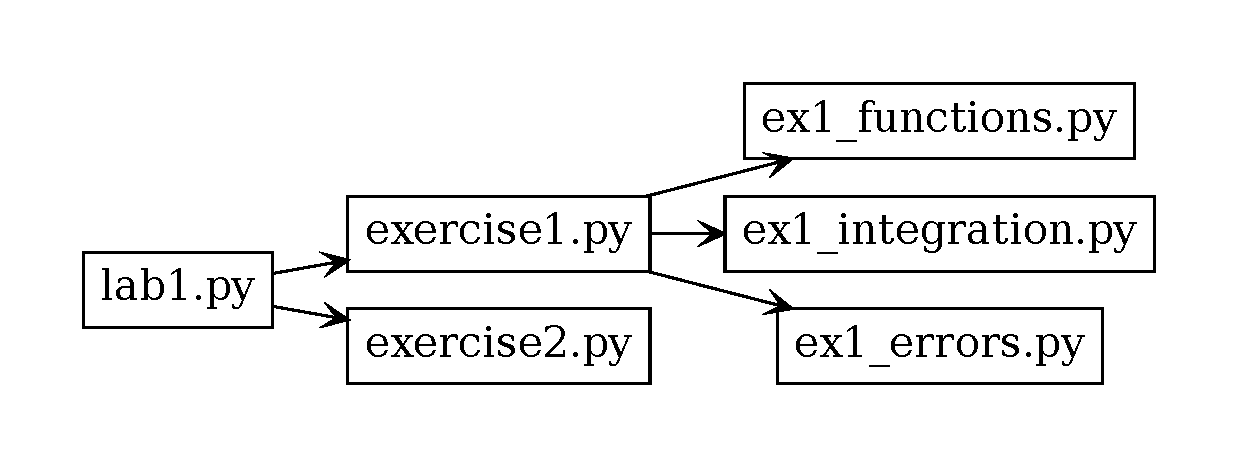
\includegraphics[width=0.5\textwidth]{figures/files}
  \caption{\label{fig:files} Exercise files dependencies. In this lab, you will
    be modifying \fileref{exercise1.py}, \fileref{ex1\_functions.py},
    \fileref{ex1\_integration.py},\fileref{ex1\_errors.py} and
    \fileref{exercise2.py}. It is recommended to check out
    \fileref{exercise1.py} before looking into the other \fileref{ex1\_*.py}
    files.}
\end{figure}

\newpage
\section*{Question 1: Numerical integration}

\subsection*{1.a Compute the analytical solution x(t) % chktex 36
  for the following linear dynamical system. Provide here the calculation steps,
  then implement the solution in
  \fileref{ex1\_fun\-ctions.py::ana\-lytic\_fun\-ction()} % chktex 36
  and run \fileref{exercise1.py} to plot the result.}

\begin{equation}
  \label{eq:ode-1}
  \dot{x} = 2 \cdot (5 - x), \quad x(t=0)=1
\end{equation}



\corr{\begin{equation}
    \label{eq:ode-1-corr}
    \begin{aligned}
      && {dx \over dt} \quad &= \quad 2 \cdot (5 - x) && \\
      \Rightarrow && {1 \over 5 - x} dx \quad &= \quad 2 dt && \\
      \Rightarrow && \int_{x_0}^x {1 \over 5-x} dx \quad &= \quad \int_{t_0}^t 2 dt && \\
      \Rightarrow && -\ln(5-x) + \ln(5-x_0) \quad &= \quad 2(t-t_0) + C && \\
      \Rightarrow && \ln({5-x \over 5-x_0}) \quad &= \quad -2(t-t_0) - C && \\
      \Rightarrow && {5-x \over 5-x_0} \quad &= \quad e^{-2(t-t_0)-C} && \\
      \Rightarrow && x(t) \quad &= \quad 5 - (5-x_0)e^{-2(t-t_0)-C} &&
    \end{aligned}
  \end{equation}
}

\corr{Using $ x_0 = 1 $ at time $ t_0 = 0 $, we obtain $ C = 0 $, thus:}
\\
\corr{\begin{equation}
    \label{eq:ode-1-corr-final}
    \begin{aligned}
      \Aboxed{x(t) = 5 - 4e^{-2t}}
    \end{aligned}
  \end{equation}
}

\corr{Python code: \texttt{x\_correct = 5--4*np.exp(-2*t)}} % chktex 36

\newpage
\subsection*{1.b In some cases, an ODE system may not have an analytical
  solution or it may be difficult to compute. Implement Euler integration in
  \fileref{ex1\_integ\-ration.py::eu\-ler\_int\-eg\-rate()}, % chktex 36
  then run \fileref{exer\-cise1.py} again to compare the solution of
  \texttt{eu\-ler\_integr\-ate()} (with 0.2 timestep) % chktex 36
  to the analytical solution obtained previously and include a figure of the
  result here. Make sure to also implement
  \fileref{ex1\_fun\-ctions.py::fun\-ction()} % chktex 36
  so that the code may be run correctly. \\ As a code template, check out
  \fileref{ex1\_integ\-ration.py::eu\-ler\_exam\-ple()}.}




% \corr{See Figure~\ref{fig:ode-integration}}

\begin{figure}[H]
  \centering 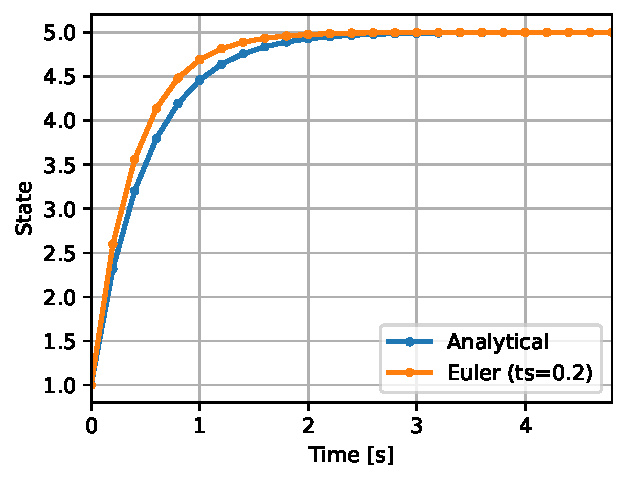
\includegraphics[height=0.4\textheight]{figures/Euler_integration}
  \caption{\corr{We can see that Euler integration with a 0.2 time steps
      approximately corresponds to the analytical
      solution.\label{fig:ode-integration}}}
\end{figure}

\corr{By computing the average abosulute error using:}

\corr{\begin{equation}
    \label{eq:average_error}
    err = {1 \over N} \sum_{_i=1}^N \left| f_{method}(i) - f_{analytical}(i) \right|
  \end{equation}
}

\corr{with N being the number of state samples, the method being Euler in this
  case and $ f_{analytical}() $ being the equation given by
  \ref{eq:ode-1-corr-final}. According to this equation, we obtain an average
  error of $ \sim 0.085 $ for the Euler method in this case. We also obtain a
  maximum absolute error of $ \sim 0.357 $.}



\clearpage

\subsection*{1.c Various efficient libraries are available to facilitate ODE
  integration, such as Scipy. In this exercise first implement your own Runge-Kutta 4th order
  method (in \fileref{ex1\_integ\-ration.py::ode\_intg\-rate\_rk()}). % chktex 36
  Then use scipy.odeint Lsoda method (in \fileref{ex1\_integ\-ration.py::ode\_intg\-rate()}) % chktex 36
  and scipy.ode adaptive Runge-Kutta Dopri method of order 4(5) (in \fileref{ex1\_integ\-ration.py::ode\_intg\-rate\_dopri()}) % chktex 36
  and solve the ode (overimpose plots of the solution using different methods and markers).
  Compare all these methods (euler, runge-kutta, lsoda and dopri) by defining an error
  function (there are multiple ways you could do this, choose an appropriate method
  and explain why) and number of time steps.
  }




\begin{figure}[H]
  \centering
  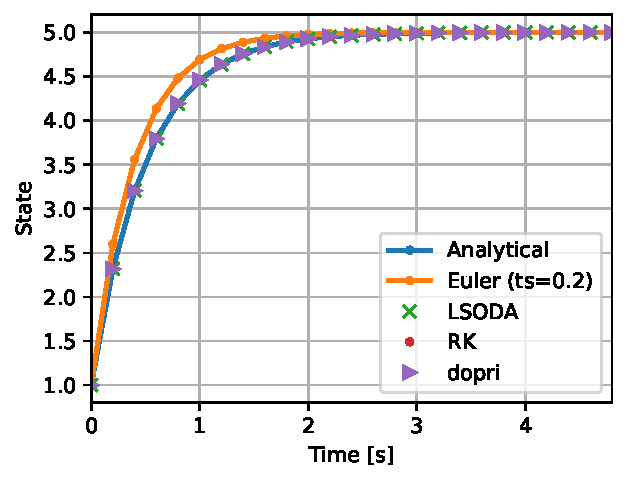
\includegraphics[height=0.4\textheight]{figures/Integration_methods}
  \caption{\corr{The Euler, Runge-Kutta and LSODA integration methods plotted
      and compared to the analytical solution\label{fig:ode-integration-rk}}}
\end{figure}

\corr{
  \begin{table}[H]
    \centering
    \begin{tabular}{ r c c c }
      \hline
      \textbf{Method} & \textbf{Average error} & \textbf{Max error} & \textbf{\# Timesteps} \\
      \hline \hline
      Euler & $ \sim 0.085 $ & $ \sim 0.357 $ & 25 \\
      Runge-Kutta & $ \sim 0.0001 $ & $ \sim 0.0004 $ & 25 \\
      dopri & $ \sim 6.41\mathrm{e}{-8} $ & $ \sim 1.43\mathrm{e}{-7} $ & Adaptive \\
      LSODA & $ \sim 1.17\mathrm{e}{-8} $ & $ \sim 5.79\mathrm{e}{-8} $ & Adaptive \\
      \hline
    \end{tabular}
    \caption{\corr{Error analysis for different integration methods}}
    \label{tab:error_analysis}
  \end{table}
}


\corr{Maintaining the 0.2 time step from the previous exercise, we observe that
  the error is much smaller using the Runge-Kutta method for a same number of
  integration times steps (25). The LSODA and dopri also obtains small error values
  similarly to the Runge-Kutta method, although this algorithm uses an adaptive
  time step which allows to control the tolerance on the error, at the cost of
  additional computation.
  }


\clearpage

\subsection*{1.d The error comparison between Euler and Runge-Kutta of question 1.c is
  not fair for the Euler method.  Briefly say why. Choose another number of time
  steps for the Euler method that is fairer when compared to
  Runge-Kutta. Provide the error values, number of time steps, and include a
  figure comparing the two integration methods. Briefly discuss which
  integration method is best.}




\begin{figure}[H]
  \centering
  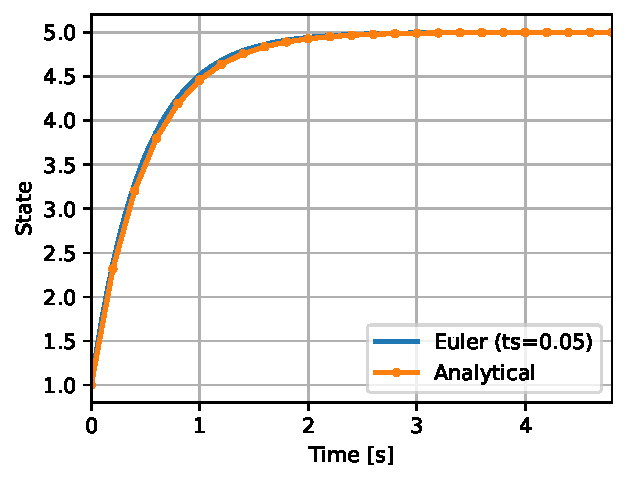
\includegraphics[height=0.4\textheight]{figures/Integration_methods_smaller_ts}
  \caption{\corr{Euler integration using smaller time step
      ($ts=0.05$)}\label{fig:ode-integration-small-ts}}
\end{figure}

\corr{The Runge-Kutta integration method computes the derivatives 4 times at
  each iteration. A fair comparison is therefore to make 4 Euler steps for each
  Runge-Kutta step.}

\corr{
  \begin{table}[H]
    \centering
    \begin{tabular}{ r c c c }
      \hline
      \textbf{Method} & \textbf{Average error} & \textbf{Max error} & \textbf{\# Timesteps} \\
      \hline \hline
      Euler & $ \sim 0.085 $ & $ \sim 0.357 $ & 25 \\
      Runge-Kutta & $ \sim 0.0001 $ & $ \sim 0.0004 $ & 100 \\
      dopri & $ \sim 6.41\mathrm{e}{-8} $ & $ \sim 1.43\mathrm{e}{-7} $ & Adaptive \\
      LSODA & $ \sim 1.17\mathrm{e}{-8} $ & $ \sim 5.79\mathrm{e}{-8} $ & Adaptive \\
      Euler (smaller ts) & $ \sim 0.020 $ & $ \sim 0.077 $ & 100 \\
      \hline
    \end{tabular}
    \caption{\corr{Error analysis for different integration methods including
        smaller Euler integration with smaller time step}}
    \label{tab:error_analysis_2}
  \end{table}
}

\corr{The error is still much smaller using Runge-Kutta time steps (ode45), even
  if approximately the same number of derivatives are computed with both methods
  (100 times for Euler, $ 25 \cdot 4 = 100 $ times for Runge-Kutta).}


\clearpage

\subsection*{1.e Test the role of the step size by plotting the integration
  error as a function of step size. You can use
  \fileref{ex1\_errors.py::com\-pute\_err\-or()} % chktex 36
  to do this by completing the code in
  \fileref{ex1\_errors.py::error()}. % chktex 36
  How accurate is the solution compared to the analytical solution for different
  step sizes?  Include here a graph showing the error against the step
  size. Explain which error measure you used (there are several options). The error of
  the adaptive solvers can be reduced by setting a smaller value of the relative
  tolerance of the solver (rtol). Reduce rtol and check the solver's accuracy. }




\begin{figure}[H]
  \centering
  \begin{subfigure}[b]{0.49\textwidth}
    \centering 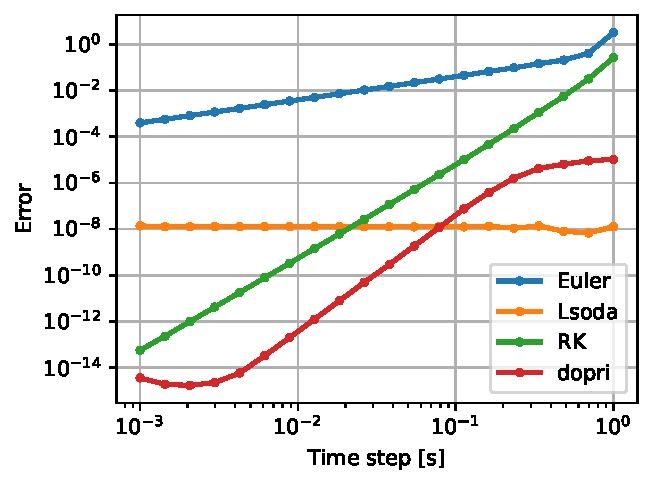
\includegraphics[width=1.0\textwidth]{figures/L1}
    \caption{\corr{L1}\label{fig:ode-err-1}}
  \end{subfigure}
  \begin{subfigure}[b]{0.49\textwidth}
    \centering 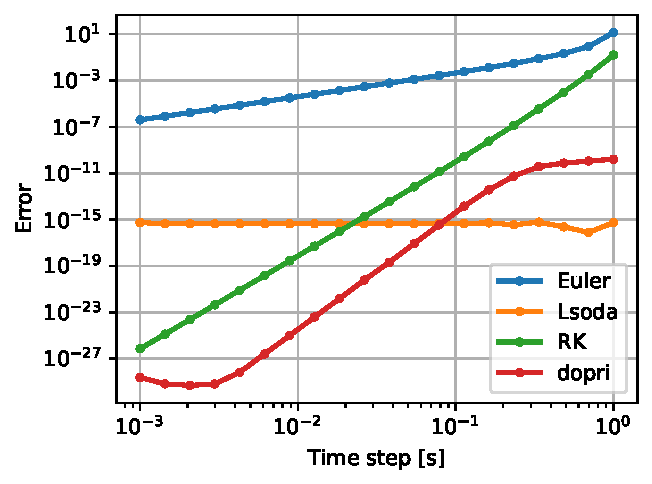
\includegraphics[width=1.0\textwidth]{figures/L2}
    \caption{\corr{L2}\label{fig:ode-err-2}}
  \end{subfigure}
  \begin{subfigure}[b]{0.49\textwidth}
    \centering 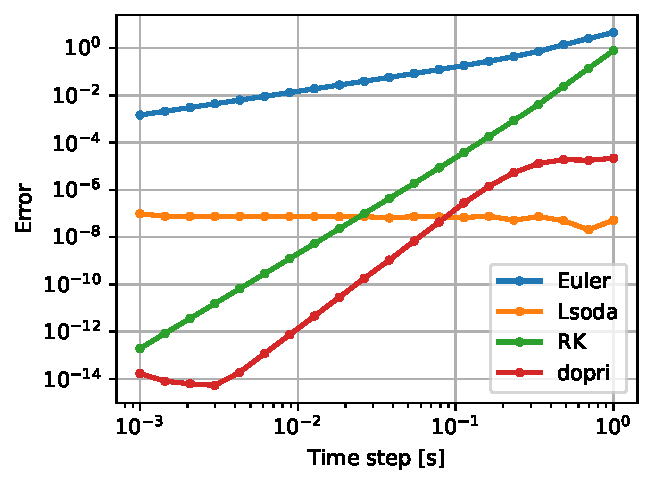
\includegraphics[width=1.0\textwidth]{figures/Linf}
    \caption{\corr{Linf}\label{fig:ode-err-3}}
  \end{subfigure}
  \caption{\corr{Error in function of time step}\label{fig:ode-step}}
\end{figure}

\corr{\begin{equation}
    \label{eq:L1}
    err_{L1} = {1 \over N} \sum_{_i=1}^N \left| f_{method}(i) - f_{analytical}(i) \right|
  \end{equation}
}

\corr{\begin{equation}
    \label{eq:L2}
    err_{L2} = {1 \over N} \sum_{_i=1}^N \left( f_{method}(i) - f_{analytical}(i) \right)^2
  \end{equation}
}

\corr{\begin{equation}
    \label{eq:Linf}
    err_{Linf} = max \left( \left| f_{method}(i) - f_{analytical}(i) \right| \right)
  \end{equation}
}

\corr{
  The Lsoda method uses a fixed L1 error tolerance of $rtol \sim 1e-8$. The dopri method uses
  a higher rtol=1e-4. In both cases the tolerance is reached by the solver and can be
  reduced by changing rtol.
}



\clearpage

\section*{Question 2: Stability analysis}

\subsection*{2.a Find the fixed points of the following linear dynamical system,
  and analyze their stability (briefly describe the calculation steps).}

\begin{equation}
  \label{eq:system}
  \dot{x} = A x,
  \qquad
  A =
  \begin{pmatrix}
    \begin{array}{rr}
      1 & 4 \\
      -4 & -2
    \end{array}
  \end{pmatrix}
\end{equation}




\corr{Fixed point $ \vec{x_o} $:}

\corr{\begin{equation}
    \label{eq:system-fixed-point}
    \begin{gathered}
      \begin{aligned}
        \dot{\vec{x_0}} = \vec{0} =
        \begin{pmatrix}
          \begin{array}{rr}
            1 & 4 \\
            -4 & -2
          \end{array}
        \end{pmatrix}
        \vec{x_o}
      \end{aligned}
      \\
      \begin{aligned}
        \quad\Rightarrow\quad \Aboxed{ \vec{x_o} =
          \begin{pmatrix}
            0 \\ 0
          \end{pmatrix}
        }
      \end{aligned}
    \end{gathered}
  \end{equation}
}

\corr{Eigenvalues $ \lambda $:}

\corr{\begin{equation}
    \label{eq:system-eigenvalues}
    \begin{gathered}
      \begin{aligned}
        && \det(A-\lambda I) &= 0 && \\
        \Rightarrow&& \det
        \begin{pmatrix}
          \begin{array}{rr}
            1 - \lambda & 4 \\
            -4 & -2 - \lambda
          \end{array}
        \end{pmatrix}
        &= 0  && \\
        \Rightarrow&& (1-\lambda) (-2-\lambda) + 16 &= 0 && \\
        \Rightarrow&& \lambda^2+\lambda+14 &= 0 &&
      \end{aligned} \\
      \begin{aligned}
        \Aboxed{ \lambda^\pm = % chktex 1 chktex 8
          {-1 \pm \sqrt{1 - 4 \cdot 14} \over 2} % chktex 1 chktex 8
          = - {1 \over 2} \pm {{\sqrt{-55} \over 2}}} % chktex 1 chktex 8
      \end{aligned}
    \end{gathered}
  \end{equation}
}

\corr{\textbf{The fixed point is stable} because the real part of both
  eigenvalues are smaller than 0.} \\ \corr{Non-zero imaginary part: the system
  exhibits \textbf{(damped) oscillations}.}


\clearpage

\subsection*{2.b Perform numerical integration from different initial conditions
  to verify the stability properties. See \fileref{exercise2.py::exercise2()}
  for implementation. Include some figures with these different time evolutions
  and their corresponding phase portrait and explain their roles.}


\begin{figure}[H]
  \centering
  \begin{subfigure}[b]{0.49\textwidth}
    \centering
    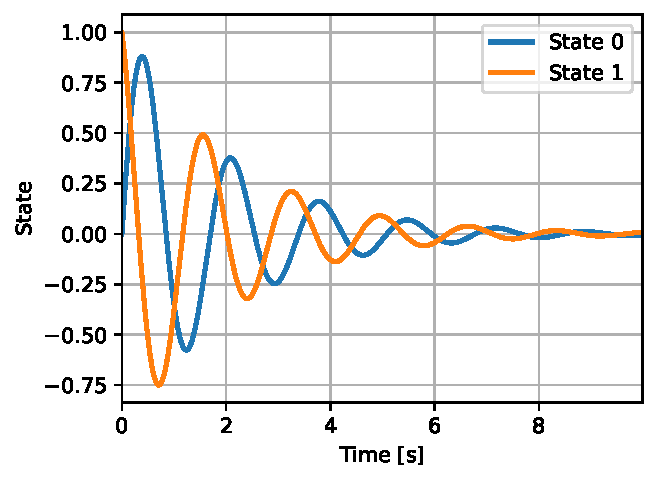
\includegraphics[width=1.0\textwidth]{figures/system_integration_state}
    \caption{\label{fig:pend-state} State}
  \end{subfigure}
  \begin{subfigure}[b]{0.49\textwidth}
    \centering
    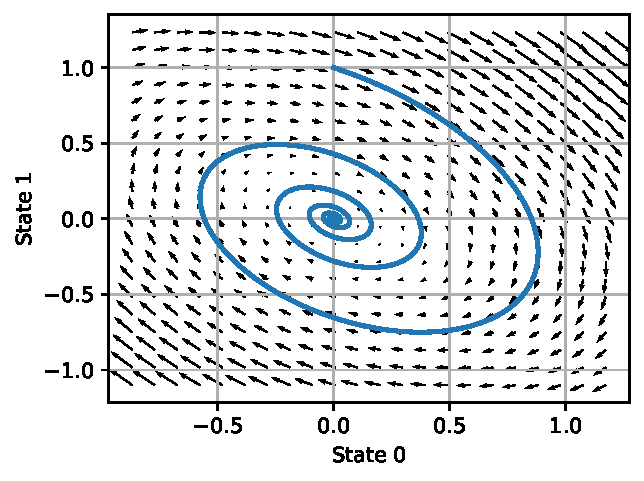
\includegraphics[width=1.0\textwidth]{figures/system_integration_phase}
    \caption{\label{fig:pend-phase} Phase}
  \end{subfigure}
  \caption{\corr{The left graph shows typical oscillations with decreasing
      amplitude (damped oscillations) in function of time. The right graph shows
      the evolution of both states, but the time information is
      lost.}\label{fig:system-pendulum}}
\end{figure}

\corr{The damped oscillations correspond to an inward spiral in the phase
  plane. The quiver plot is a vector plot that shows the general behavior of the
  system in the phase plane.}

\begin{figure}[H]
  \centering
  \begin{subfigure}[b]{0.49\textwidth}
    \centering 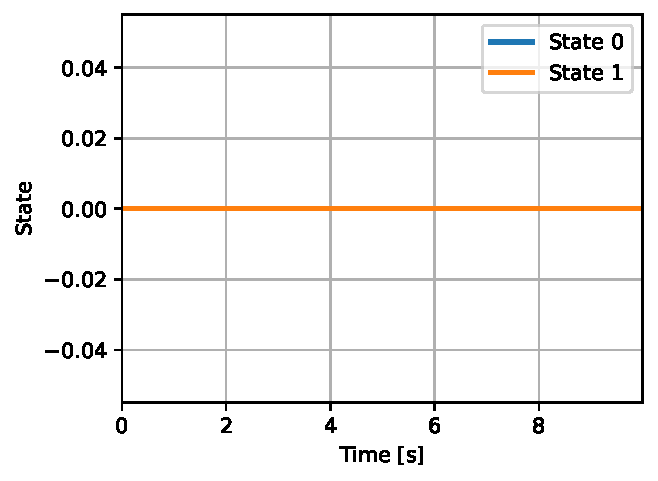
\includegraphics[width=1.0\textwidth]{figures/stable_state}
    \caption{\label{fig:pend-stable-state} State}
  \end{subfigure}
  \begin{subfigure}[b]{0.49\textwidth}
    \centering 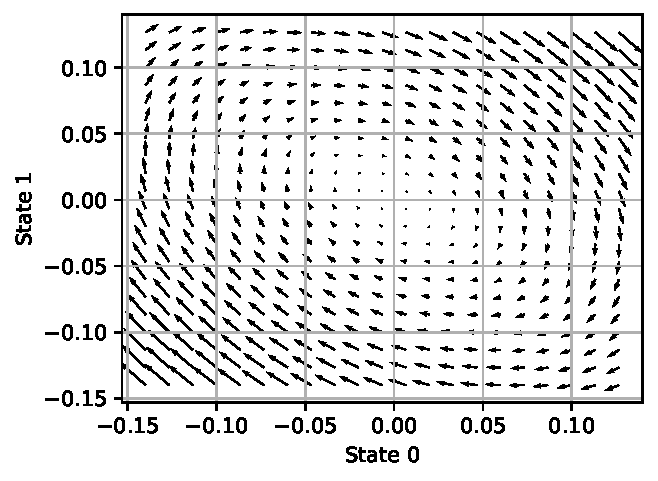
\includegraphics[width=1.0\textwidth]{figures/stable_phase}
    \caption{\label{fig:pend-stable-phase} Phase}
  \end{subfigure}
  \caption{\corr{These graphs show the evolution of the system from (0,0) to
      demonstrate the fixed point behavior.}\label{fig:pend-stable}}
\end{figure}


\clearpage

\subsection*{2.c Change one value in matrix A such that the time evolution
  becomes periodic for some initial conditions. Say which value and include a
  time evolution figure.}




\corr{In order for the system to become periodic, we need the eigenvalues
  $\lambda$ to be purely imaginary, say by modifying the first element of the
  matrix:}

\corr{\begin{equation}
    \label{eq:system-periodic-eigenvalues}
    \begin{gathered}
      \begin{aligned}
        && \det(A-\lambda I) &= 0 && \\
        \Rightarrow&& \det
        \begin{pmatrix}
          \begin{array}{rr}
            a - \lambda & 4 \\
            -4 & -2 - \lambda
          \end{array}
        \end{pmatrix}
        &= 0  && \\
        \Rightarrow&& (a-\lambda) (-2-\lambda) + 16 &= 0 && \\
        \Rightarrow&& \lambda^2+(2-a)\lambda+(16-2a) &= 0 &&
      \end{aligned} \\
      \begin{aligned}
        \lambda^\pm = {-(2-a) \pm \sqrt{(2-a)^2 - 4 \cdot (16 - 2a)} \over 2}
      \end{aligned}
    \end{gathered}
  \end{equation}
}

\corr{By selecting $ a = 2 $, we obtain:}

\corr{\begin{equation}
    \label{eq:system-periodic-eigenvalues-results}
    \lambda^\pm = {-(2-2) \pm \sqrt{(2-2)^2 - 4 \cdot (16 - 4)} \over 2} = \pm \sqrt{12} j
  \end{equation}
}

\corr{Thus the system changed to:}

\corr{
  \begin{equation}
    \label{eq:system-periodic}
    \dot{x} = A x,
    \qquad
    A =
    \begin{pmatrix}
      \begin{array}{rr}
        2 & 4 \\
        -4 & -2
      \end{array}
    \end{pmatrix}
  \end{equation}
}

\begin{figure}[H]
  \centering
  \begin{subfigure}[b]{0.49\textwidth}
    \centering 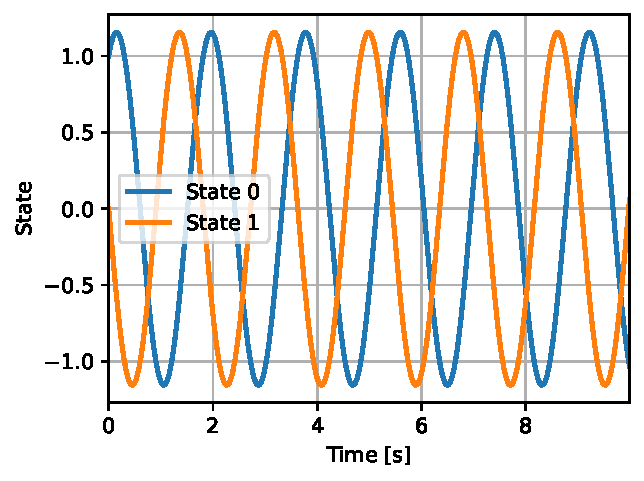
\includegraphics[width=1.0\textwidth]{figures/periodic_state}
    \caption{\label{fig:pend-periodic-state} State}
  \end{subfigure}
  \begin{subfigure}[b]{0.49\textwidth}
    \centering 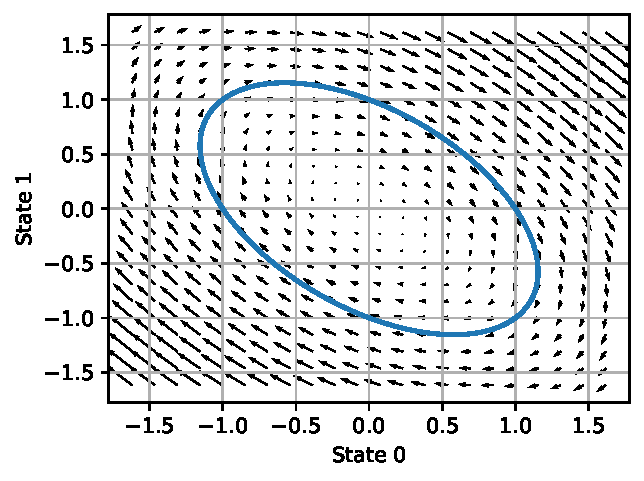
\includegraphics[width=1.0\textwidth]{figures/periodic_phase}
    \caption{\label{fig:pend-periodic-phase} Phase}
  \end{subfigure}
  \caption{\corr{A is changed to: A = [[2,4],[-4,-2]] Eigen values are now
      complex numbers with real part = 0. This leads to oscillatory behavior
      without damping.}\label{fig:pend-periodic}}
\end{figure}


\clearpage

\subsection*{2.d Compute the eigenvalues and eigenvectors of the following system.
What can you say about the stability of its fixed point? What is the meaning of its
eigenvectors? Try to plot the flow of the system to get an intuition of its behavior.}

  \begin{equation}
    \label{eq:saddle-system}
    \dot{x} = A x,
    \qquad
    A =
    \begin{pmatrix}
      \begin{array}{rr}
        1 & 1 \\
        4 & -2
      \end{array}
    \end{pmatrix}
  \end{equation}



\corr{The first part of the exercise is solved as in 2.c.}

  \corr{Eigenvalues $ \lambda $:}

  \corr{\begin{equation}
      \label{eq:saddle-system-eigenvalues}
      \begin{gathered}
        \begin{aligned}
          && \det(A-\lambda I) &= 0 && \\
          \Rightarrow&& \det
          \begin{pmatrix}
            \begin{array}{rr}
              1 - \lambda & 1 \\
              4 & -2 - \lambda
            \end{array}
          \end{pmatrix}
          &= 0  && \\
          \Rightarrow&& (1-\lambda) (-2-\lambda) - 4 &= 0 && \\
          \Rightarrow&& \lambda^2+\lambda-6 &= 0 &&
        \end{aligned} \\
        \begin{aligned}
          \Aboxed{ \lambda^\pm = % chktex 1 chktex 8
            {-1 \pm \sqrt{1 + 4 \cdot 6} \over 2} % chktex 1 chktex 8
            = - {1 \over 2} \pm {{5 \over 2}}} % chktex 1 chktex 8
        \end{aligned}
      \end{gathered}
    \end{equation}
  }

  \corr{The eigenvalues of the system are equal to $ \lambda_{1} $ = 2 and $ \lambda_{2} $ = -3\\
  \textbf{The fixed point is a saddle node} because the real part of one
    eigenvalue is greater than 0.}

  \corr{Eigenvectors $ \vec{v} $:\\
  Note that the matrix is singular, therefore we just consider one of the two equations.\\
  There are infinite solutions to the system, we will consider vectors with unitary
  norm.}

  \corr{\begin{equation}
      \label{eq:saddle-system-eigenvector1}
      \begin{gathered}
        \begin{aligned}
          && (A-\lambda_1 I)\vec{v_1} &= 0 && \\
          \Rightarrow&&
          (A-2 I)\vec{v_1} &= 0 && \\
          \Rightarrow&&
          \begin{pmatrix}
            \begin{array}{rr}
              -1 & 1 \\
              4 & -4
            \end{array}
          \end{pmatrix}
          &\vec{v_1}= 0  && \\
          \Rightarrow&&
            v_{1x} &= v_{1y} && \\
        \end{aligned} \\
        \begin{aligned}
          \Aboxed{ \vec{v_1} = % chktex 1 chktex 8
          \begin{pmatrix}
            \begin{array}{rr}
              1/\sqrt{2} \\
              1/\sqrt{2}
            \end{array}
          \end{pmatrix}
          }
        \end{aligned}
      \end{gathered}
    \end{equation}
  }

  \corr{\begin{equation}
    \label{eq:saddle-system-eigenvector2}
    \begin{gathered}
      \begin{aligned}
        && (A-\lambda_2 I)\vec{v_2} &= 0 && \\
        \Rightarrow&&
        (A+3 I)\vec{v_2} &= 0 && \\
        \Rightarrow&&
        \begin{pmatrix}
          \begin{array}{rr}
            4 & 1 \\
            4 & 1
          \end{array}
        \end{pmatrix}
        &\vec{v_2}= 0  && \\
        \Rightarrow&&
        4v_{2x} &= -v_{2y} && \\
      \end{aligned} \\
      \begin{aligned}
        \Aboxed{ \vec{v_2} = % chktex 1 chktex 8
        \begin{pmatrix}
          \begin{array}{rr}
            1/\sqrt{17} \\
            -4/\sqrt{17}
          \end{array}
        \end{pmatrix}
        }
      \end{aligned}
    \end{gathered}
  \end{equation}
}

\clearpage

\corr{You can observe in Figure~\ref{fig:saddle-system-state} how the eigenvector associated to the negative value corresponds
to a line of stable solutions (the stable manifold). Due to the uniqueness theorem, trajectories
cannot cross, therefore the stable manifold is effectively dividing the phase space in two regions.
Points starting on the left of the manifold will diverge towards ($ -\inf, -\inf $), points
starting on the right of the manifold will diverge towards ($ +\inf, +\inf $).  }


\begin{figure}[H]
  \centering
  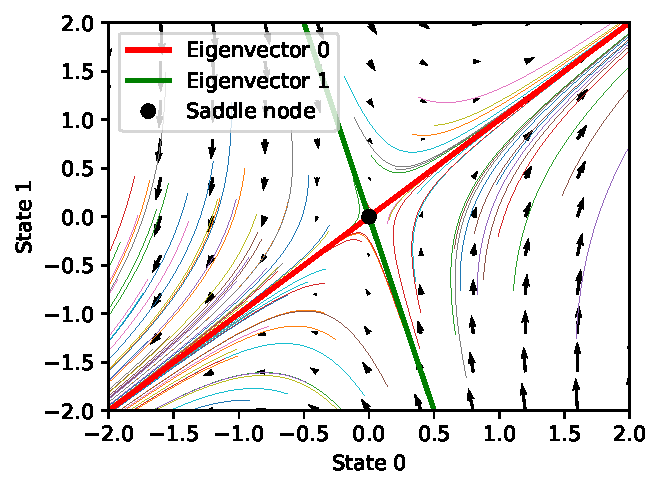
\includegraphics[width=1.0\textwidth]{figures/saddle_node_phase_diagram}
  \caption{ \corr{Phase diagram of the system with a saddle point.
  The eigenvalues of the saddle point correspond to the stable and unstable manifold of the system} }
  \label{fig:saddle-system-state}
\end{figure}


\end{document}